\chapter{Background}
\label{chapter:background}

\section{Ethereum}
    \subsection{Smart Contract}
        Ethereum~\cite{buterin2014next} was proposed in 2014 by Vitalik Buterin, it is a decentralized, open-source blockchain, and it also supports smart contracts. Because Ethereum enables smart contracts, the programmers can build their distributed applications by writing smart contract programs, e.g., Solidity. With smart contract technology, they can build self-enforce, self-verify and tamper-proof systems, such as voting systems, healthcare, supply chain, financial service, and so on. \par        
        In the Etheruem platform, the block not only stores transaction records, but also stores smart contract so that Ethereum has the capability to compute business logic. The blockchain uses Merkle tree to store the transactions in every block.\par

    \subsection{Merkle tree}
    \begin{figure}[hb]
        \centering
        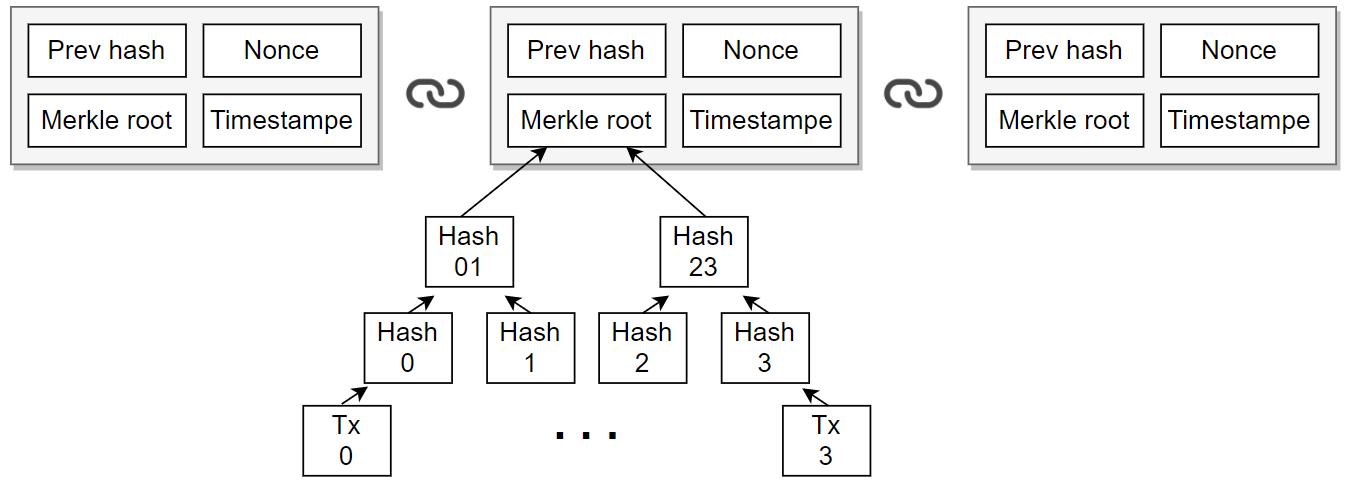
\includegraphics[height=!,width=1\linewidth,keepaspectratio=true]{figures/merkle_tree_in_BC.png}
        \caption{{\footnotesize Merkle tree in Bitcoin blockchain}}
        \label{fig:merkleTreeInBC}
    \end{figure}
    Merkle trees are important in blockchain technology. A Merkle tree is a tree in which every node is stored with the hash of data. Each node is the hash of his leaves. In Bitcoin blockchain, it uses the Merkle tree as proof to make sure the data block can't be tampered with, it is not possible to modify the data after the data written in the blockchain as shown Figure~\ref{fig:merkleTreeInBC}.\par
    \begin{figure}[htb]
        \centering
        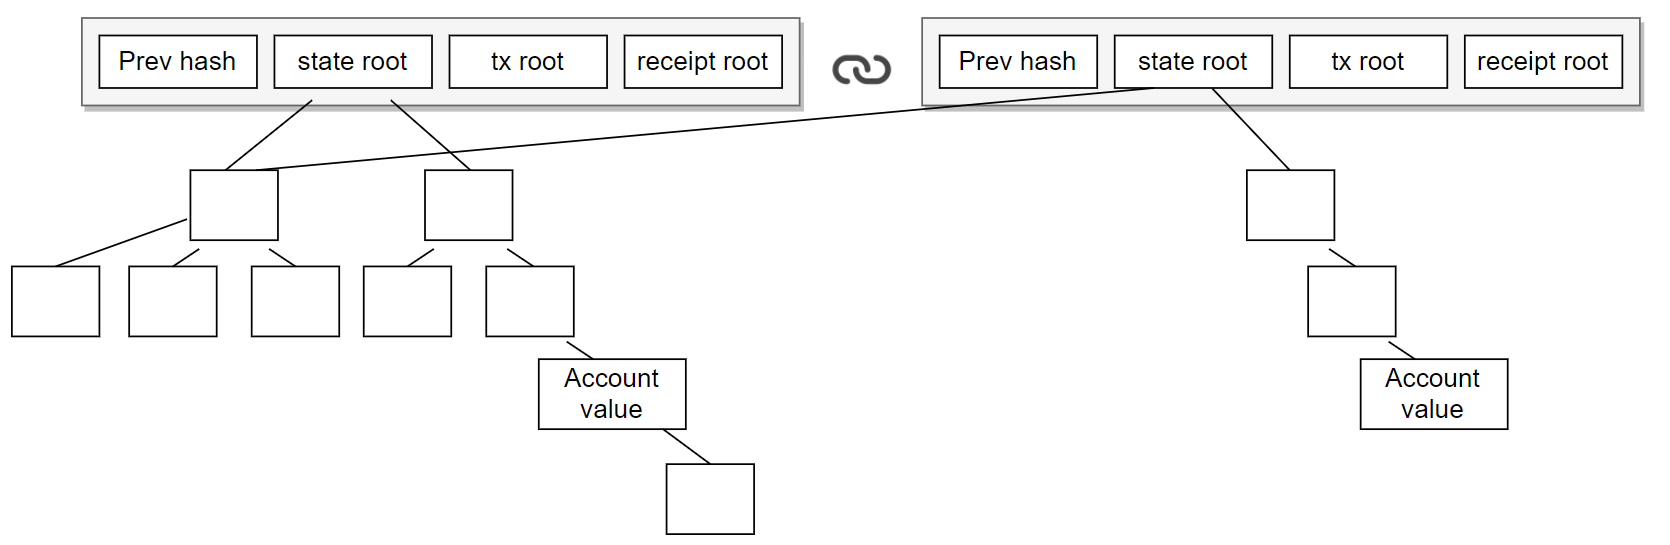
\includegraphics[height=!,width=1\linewidth,keepaspectratio=true]{figures/merkle_tree_in_Eth.png}
        \caption{{\footnotesize Merkle tree in Ethereum}}
        \label{fig:merkleTreeInEth}
    \end{figure}
    The Merkle tree in Ethereum is as Figure~\ref{fig:merkleTreeInEth}. Every block header has not only one tree, but three trees for transactions, receipts, and state. The state root is the root hash of the Merkle Patricia tree that used to store the entire state of the Ethereum blockchain, like account balances, contract storage, and contract code. Unlike Bitcoin blockchain, Ethereum uses Merkle Patricia tree as the state tree, it consists of a map struct, the keys are account address and the values are account declarations such as the balance, nonce.

    \subsection{Elliptic Curve Cryptography (ECC)}
        Elliptic Curve Cryptography is public key cryptography based on elliptic curves. In Ethereum, they use ECC to generate the key pair. Initially, the base point \(G\) on elliptic curve \(CURVE\) must be provided, and then randomly generate 256-bits integer \(m\) as a private key which is used to sign message or transaction. If given \(m\), it is easy and fast to find 512-bits public key \(P\). But if given \(P\), it is impossible to find \(m\) because of Elliptic Curve Logarithm Problem. The Ethereum address is the last 20-bytes of  Keccak-256 hash of the public key.\par

        \begin{equation}
            P=[m]G
        \end{equation}

        Elliptic Curve Digital Signature Algorithm (ECDSA) is used to create a digital signature of data that uses elliptic curve cryptography. ECDSA isn't used to encrypt any data, it makes sure that the data was not tampered with. In the Ethereum blockchain, it used to prove ownership of an address without revealing private key. \par
        After signing message using ECDSA through private key, the digital signature consists of three values: \(r, s, v\). \(r\) and \(s\) are the values used in standard ECDSA signatures, and \(v\) means recover id that used to recover signed message. In blockchain (e.g., Bitcoin, Ethereum), we called it public key recovery. If we get \((r, s)\) and message, we can compute the public key to verify message.\par
        
    \section{MetaMask}
        \begin{figure}[htb]
            \centering
            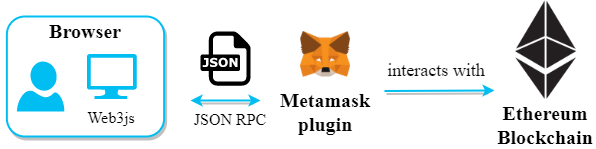
\includegraphics[height=!,width=1\linewidth,keepaspectratio=true]{figures/architecture_of_dapp.png}
            \caption{{\footnotesize Architecture of DApp}}
            \label{fig:architecture_of_dapp}
        \end{figure}
        MetaMask~\cite{metamask} is the most popular crypto wallet for accessing Ethereum distributed application (DApp). This tool can enable web3 API in website so that users can interact with various Etehereum blockchain from Javascript~\cite{web3.js}, e.g., Mainnet, Testnet. It also creates accounts by the user themself. The user of MetaMask can create and manage their accounts; moreover, MetaMask provides an interface that user can perform a transaction to the connected blockchain.\par
        Because the user securely manages owned Ethereum account through MetaMask, the user can use their private key to sign a transaction or sign data to prove ownership of an account. Using this crypto wallet, the developers of decentralized applications can build their own cryptocurrencies and focus on designing and implementing functions of smart contracts. There are several different architectures for distributed apps~\cite{wessling2018engineering}, the most common way is the developer design frontend that can allow the users to interact with the business logic by MetaMask. Or, the user can send a transaction to blockchain directly.\par
        In the MetaMask wallet, it seems to have a lot of benefits. Firstly, the keys are stored in the user's browser and it doesn't store on wallet provider's server, so the user can manage his/her private key and public key without server. Secondly, it provides an easy to use interface, every user can send and receive cryptocurrency or token.\par
        Regarding the architecture of Dapp, Figure~\ref{fig:architecture_of_dapp} shows that the web3.js libraries can enable user's browser to interact with blockchain so that users can read and write data from smart contracts, send transactions between accounts. 



\newpage

\section{OAuth}
- OAuth 2.0 flow and explain

\newpage

\section{Trust Service Provider (TSP)}
- Open Banking flow
- Current TSP in Taiwan
- Three stage table

\newpage

\section{Related works}

\subsection{Identity integration}
\subsection{Access control}
\subsection{Open banking}
In this section, we will provide an overview of related literature about blockchain-based access control, identity management, data sharing, and Open Banking ecosystem.\par
In traditional access control management, the most common solution is PKIs, but it has some concerns about scalability and granularity. Paillisse \emph{et al.}~\cite{paillisse2019distributed} presented a blockchain-based approach to address these problems. They take advantage of blockchain to record and distribute access control policies. Daraghmi \emph{et al.}~\cite{daraghmi2019medchain,daraghmi2019unichain} described a blockchain-based system for electronic medical records and academic records, using blockchain smart contract to manage the data access permission securely and effectively. It also utilizes advanced encryption techniques to protect user's privacy. 
Rouhani \emph{et al.}~\cite{rouhani2020distributed} proposed a distributed Attributed-Base Access Control (ABAC) system that can provide auditing of access attempts. This work has focused on addressing audit and scalability, moreover, they apply the solution to the digital library and improve a lot.
Fu \emph{et al.}~\cite{fu2020soteria} proposed a user rights management system that aims to protect user privacy through enforcing executable sharing agreement. They also adopted multi-layer blockchain architecture to satisfy CAP (consistency, availability, and partition tolerance) theorem.\par

More recent attention has focused on data sharing. The common scenario is Open Banking system since it needs secure identity authentication and the perfect mechanism of user data privacy. With blockchain technology, it can solve the shortcoming of the centralized system and prevent user's data from being breached.